\documentclass[12pt]{article}
\usepackage[letterpaper, portrait, margin=1in]{geometry}
\usepackage{amsfonts}
\usepackage{amsmath}
\usepackage{listings}
\usepackage{graphicx}
\usepackage{breqn}
\pagenumbering{arabic}
\usepackage{subcaption}
\usepackage{amsthm}
\usepackage{cite}
\graphicspath{{C:/Users/x92423/Documents/}}
\begin{document}
%\title{Statistical Learning in Financial Markets: \\ 
%	\large A Literature Review}
%\author{Joe Schlessinger \\ COL Grover LaPorte, MAJ(P) Tim Sikora, \& CPT Steven Morse}
%\maketitle
%\newpage

\begin{titlepage}
	\begin{center}
		\vspace*{1cm}
		
		\textbf{\large Statistical Learning in Financial Markets}
		
		\vspace{0.5cm}
		A Literature Review
		
		\vspace{1.5cm}
		
		\textbf{CDT Joseph Schlessinger \\ COL Grover LaPorte, MAJ(P) Tim Sikora, \& CPT Steven Morse}
		
		\vfill
		
		%A thesis presented for the degree of\\
		%Doctor of Philosophy
		
		\vspace{0.8cm}
		
		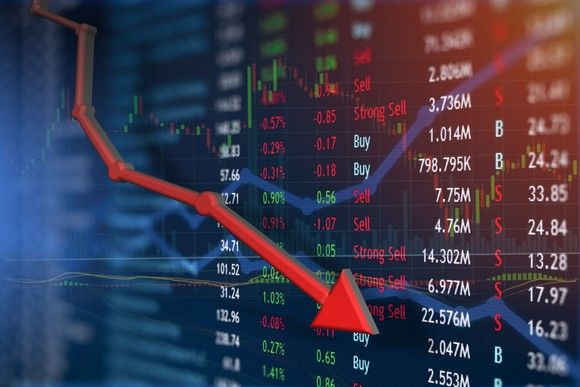
\includegraphics[width=0.8\textwidth]{stock.jpg}
		
		\vfill 
		Department of Mathematical Sciences\\
		United States Military Academy\\
		West Point, New York\\
		12 October, 2018
		
	\end{center}
\end{titlepage}

\tableofcontents
\newpage 
\section{Introduction}
For this research project, I am exploring applying statistical learning techniques to time series analysis. Specifically, I am looking at financial data, or stock prices, as the time series of interest. The following literature review will examine the basics of investing, and provide a cursory overview of the classical methods of time series analysis and machine learning.

\section{Basics of Investing}
Investing is a complicated subject. There are a number of different types of financial assets, trades, investment strategies, and risk measurements. For the purposes of this project, we will simplify financial markets significantly. 

\subsection{Stocks}
A stock is a piece of some public company. A public company means it is traded publicly; anyone may purchase a share giving them partial ownership of the company. The stock market is open from 8:00 AM to 4:00 PM, at which point differing volumes of trading occur. 

\subsection{Dollar Cost Averaging}
Dollar cost averaging is a popular investment strategy. It comes from the wisdom that the stock market is unpredictable; as in, the investor has no way of knowing what will happen. By investing some fixed amount at a regular interval, the investor averages out the risk and will gain, on average, whatever the stock makes. This phenomenon can be seen in Figure \ref{dca}. Dollar Cost Averaging is the standard of comparison for investment strategies. For this project, I am rejecting the practical wisdom that the stock market is unpredictable; through statistical learning, I hope to design an investment strategy that outperforms dollar cost averaging.

\begin{figure}[ht]
	\centering
	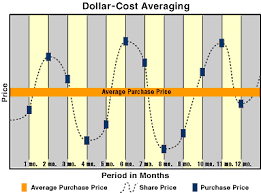
\includegraphics[width=.5\textwidth]{dca.png}
	\caption{Dollar Cost Averaging averages the purchase price of the stock over time. \cite{dca}}
	\label{dca}
\end{figure}

\subsection{Practical Assumptions}
In an effort to transform the financial world into a more wieldy dataset for academic research, I have made a few simplifying assumptions.
\begin{itemize}
	\item Trades occur instantly and at the beginning of the day. The investment algorithm purchases at the exact price the stock closed at the previous day. This is unrealistic to some extent because in order to purchase some number of shares at some price, there has to be another owner willing to sell those shares at that price, which is not always the case. However, this assumption is consistent across both the statistical investment methods and dollar cost averaging standard of comparison.
	
	\item There is no transaction fee, which is not the case when trading. Typically, investors pay some fixed fee to the brokerage firm for completing the transaction. Again, because this is a consistent assumption in the dollar cost average baseline, this will not affect the comparison.
			
\end{itemize}
\section{Time Series Analysis}
Stock data examined over time forms a time series. Explicitly, we have some series $\{X_t\} = \{x_1, x_2, \dots, x_n\}$ where $x_t$ is some $m$-dimensional vector corresponding to the $t$th day of a stock. We are concerned with forecasting the price of a stock for the next day. Given $\{X_t\}$, can we predict $x_{t+1}$?

\subsection{Stationary Models}  
A time series is stationary if it has similar statistical properties at $\{X_t\}$ and at $\{X_{t+h}\}$ for some $h$. For a more mathematically rigorous definition of stationary, we need to define some additional functions.

The mean function of $\{X_t\}$ is $\mu_X(t) = E(X_t)$. The first requirement for stationarity is that $\mu_X(t)$ be independent of $t$. 

The second requirement has to do with the covariance of the time series. The covariance function of $\{X_t\}$ is defined as
$$\gamma _X(r,s) = \text{Cov}(X_r, X_s) = E[(X_r - \mu _X(r))(X_s - \mu_X(s))]$$

Our next requirement for a time series to be stationary is that $\gamma_X(t+h, t)$ is independent of $t$ for each $h$. 

\subsection{Trends, Seasonality, and Noise}
Stock data as a time series is not stationary. This should be obvious. A time series generally has a trend component, a seasonal component, and some random noise component. Thus, a time series can be decomposed in the following way
$$X_t = m_t + s_t + Y_t$$

where $m_t$ is the trend component, $s_t$ is the seasonal component, and $Y_t$ is some random stationary noise component. In Figure \ref{trends}, these components are on display. The plot titled purely random error is our random noise component; this is a stationary time series. The plots depict two types of trend, linear and nonlinear. A trend refers to some change to the data that occurs over time. As stocks generally increase overtime, there is clearly some trend involved in stock time series. Additionally, time series can have seasonality, seen in the bottom left of the figure. Anything that is cyclic can be represented as seasonality. As an example, if a stock increased at the beginning of the month, peaked in the middle, and then decreased before bottoming out at the end of the month, this would be a seasonality we would have to negate before applying time series analysis. The plot in the bottom right demonstrates an interaction of these additive terms, which is generally what financial data looks like. \cite[22]{timeseries}

\begin{figure}[ht]
	\centering
	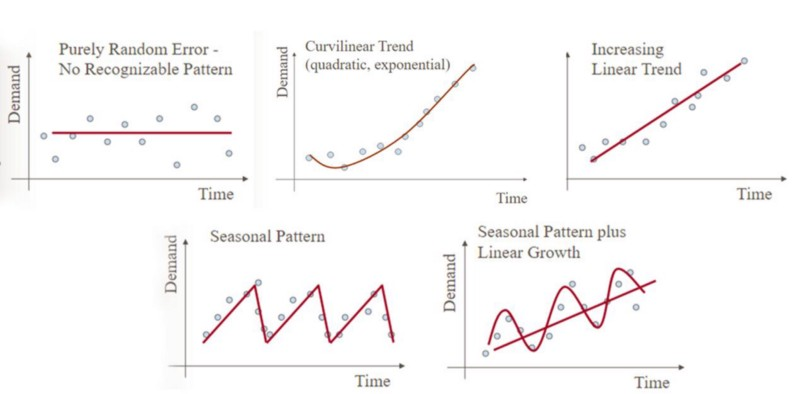
\includegraphics[width=.75\textwidth]{trend.jpeg}
	\caption{This figure shows the various components of a time series. \cite{trend}}
	\label{trends}
\end{figure}

\subsubsection{Trend and Seasonality Elimination by Differencing}
Many time series analysis models require a stationary time series. While we can account for this by attempting to estimate the trend and seasonality of the time series, in this case we will transform the data to eliminate trend and seasonality.

To eliminate trend, you can apply the difference operator $\nabla^d$ which lags the time series data by the past $d$ days.
$$\nabla^1 X_t = X_t - X_{t-1}=(1-B)X_t$$

where $B$ is the backward shift operator such that $BX_t = X_{t-1}$.

Thus, $$\nabla^t X_t = \nabla(\nabla(X_t)) = (1-B)(1-B)X_t = (1-2B+B^2)X_t = X_t-2X_{t-1}+X_{t-2}$$

This applies for some general $\nabla^d$. A similar technique can be used to negate seasonality by applying $\nabla_d$, where subscript $d$ instead refers to lagging by the value in the time series $d$ periods ago.

$$\nabla_d = X_t - X_{t-d} = (1-B^d) X_t$$

A more rigorous explanation can be found in \cite[22-32]{timeseries}.

\subsection{Moving Average}
Moving average models use the past forecast errors to model the time series and forecast. 

$$ x_{t} = c + \varepsilon_t + \theta_{1}\varepsilon_{t-1} + \theta_{2}\varepsilon_{t-2} + \dots + \theta_{q}\varepsilon_{t-q}$$

$\theta_q$ represents the weight for $\varepsilon_q$. An MA($q$) model considers the $q$ most recent data points. \cite[8.4]{forecasting}


\subsection{Autoregressive Models}
Autoregressive models use past values of the variable to predict future values of the variable. With financial data, the implication in using autoregressive models is the stock market repeats itself, and we can learn from the past what may happen in the future. \cite[8.3]{forecasting} The autoregressive model can be written as 

$$x_{t} = c + \phi_{1}x_{t-1} + \phi_{2}x_{t-2} + \dots + \phi_{p}x_{t-p} + \varepsilon_{t}$$

where $\varepsilon$ is white noise, $c$ is some intercept and $\phi_n$ is the weight associated with data point $y_n$. An AR($p$) model considers the most recent $p$ data points in the time series.

\subsection{ARIMA}
AutoRegressive Integrated Moving Average (ARIMA) combines moving average and autoregression into one model. 

$$ x'_{t} = c + \phi_{1}x'_{t-1} + \cdots + \phi_{p}x'_{t-p} + \theta_{1}\varepsilon_{t-1} + \cdots + \theta_{q}\varepsilon_{t-q} + \varepsilon_{t} $$

$x'_t$ refers to the differenced series. This comes from the "integrated" part of the model; it is differenced. The general ARIMA model is of form ARIMA($p,d,q$) where $p$ is the order of the autoregressive part, $d$ is the degree of differencing, and $q$ is the order of the moving average part. \cite[8.5]{forecasting}



\section{Machine Learning} 
At its core, machine learning is a subset of data science. Through statistical methods, we can analyze the 

\subsection{Regression v. Classification}
Machine learning breaks down into two main subsets: regression and classification. The distinction between the two subsets lies in the output type. While some models seek to predict a quantitative measurement based on the input, others may want to predict a qualitative measurement; models with quantitative outputs are regression and models with qualitative outputs are classification. \cite[9-10]{springer} When looking at stock time series data, a regression model would seek to forecast what the price of the stock will be the following day, while a classification model might seek to determine whether the stock will go up or down. 

\subsection{Linear Models}
Linear models are one of the simplest approaches to prediction. Given a vector of inputs 
$X =  \begin{bmatrix} 
x_1 \\
x_2 \\
\vdots \\
x_n
\end{bmatrix}
$, a linear model seeks to predict output using 

$$\hat{Y} = \hat{\beta}_0 + \sum_{j=1}^{p} X_j \hat{\beta}_j$$

where $\hat{\beta}$ is the intercept for the data and $\hat{\beta}_j$ are the coefficients for each input variable $X_j$. \cite[11]{springer}

The challenge is determining the coefficients. There are a number of methods that accomplish this but the most popular is least squares, which seeks to minimize the residual sum of squares. 
With least squares, we select $\hat{\beta}$ according to the following function:
$$\hat{\beta} = \text{argmin} \sum_{i=1}^{N} (y_i - B_0 - \sum_{j=1}^{p} x_{ij} \beta_j)^2$$
\cite[42]{springer}


\subsubsection{Ridge Method}
One problem that can occur with least squares regression is poor prediction accuracy because of high variance. \cite[55]{springer} This is also known as overfitting. A solution is to shrink the size of the regression coefficients by imposing a penalty on their size. This is a simple modification of the least squares coefficient selection where we determine the coefficients according to the following formula: 
$$\hat{\beta}_{\text{ridge}} = \text{argmin} \sum_{i=1}^{N} (y_i - B_0 - \sum_{j=1}^{p} x_{ij} \beta_j)^2 + \gamma \sum_{j=1}^{p}\beta_j^2$$
\cite[59]{springer}

Notice, the only difference between ridge and least squares is the penalty term for coefficient size, which is controlled by the tuning parameter $\gamma$. A large $\gamma$ will place a large penalty on parameter size. As $\gamma$ increases, the coefficients approach 0. 

\subsubsection{Lasso Method}
The Lasso method is another variant of least squares that employs a slightly different penalty. Coefficient selection goes according to the following equation:
$$\hat{\beta}_{\text{lasso}} = \text{argmin} \sum_{i=1}^{N} (y_i - B_0 - \sum_{j=1}^{p} x_{ij} \beta_j)^2 + \gamma \sum_{j=1}^{p}|\beta_j|$$

With lasso, the penalty is $|\beta|$ instead of $\beta^2$. One effect of using this different penalty is a sufficiently large $\gamma$ will lead to some coefficients equaling zero. The lasso method thus does variable selection in addition to fitting a linear model. \cite[64]{springer}

\subsection{Neural Networks}
Neural networks are a type of nonlinear statistical model. Neural networks have three parts: an input layer, which takes the same vector $X$, a hidden layer which performs some, and an output layer. Assume we have $I$ input nodes, $J$ hidden layer nodes, and $K$ output nodes. The following explanation corresponds to Figure \ref{neuralnet}. 

\begin{figure}[ht]
	\centering
	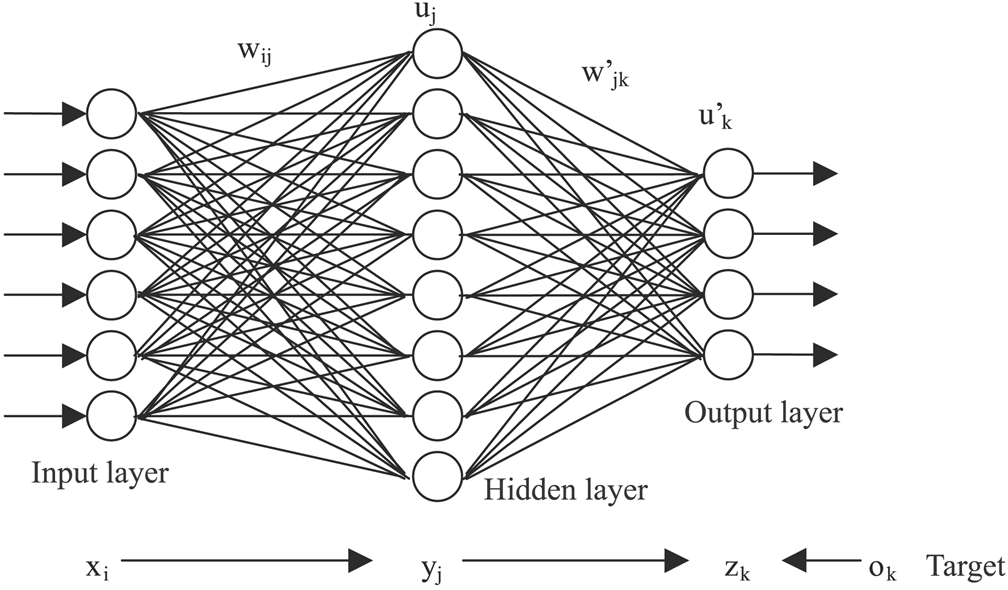
\includegraphics[width=.85\textwidth]{NeuralNetwork.png}
	\caption{This is a visual depiction of a general neural net. Note, for regression, there is a single output node. \cite{neural}}
	\label{neuralnet}
\end{figure}

Each hidden layer node $u_j$ learns a vector of weights $\alpha_j$ and some bias $\alpha_{0j}$. Bias in neural networks is simply some intercept for the vector of weights $\alpha_j$. Each weight $\alpha_{ji}$ corresponds to an input node $X_i$. Note, the hidden layer captures certain features of the model, but the weights and values do not have an obvious meaning. It is for this reason that neural networks are mysterious and often thought of as a black box. The value of $u_j$ is simply some function $\sigma$ applied to a linear combination of the weights and input values:

$$u_j = \sigma(\phi_{j} + \sum_{x=0}^{i}\alpha_{ji} X_i)$$

$\sigma(v)$ is referred to as the activation function, which is often chosen to be the sigmoid function:
$$\sigma(v) = \frac{1}{1+e^{-v}}$$
The sigmoid function simply takes an input $v$ and maps it between 0 and 1, as seen in Figure \ref{sigmoid}. 

\begin{figure}[ht]
	\centering
	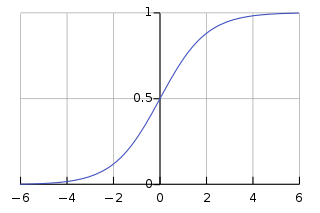
\includegraphics[width=.5\textwidth]{sigmoid.png}
	\caption{The sigmoid function is often used as the activation function in hidden layer nodes.}
	\label{sigmoid}
	
\end{figure}

From this set of hidden layer values $U = \{u_j\}$, we can generate output.

Each output node $u'_k$ has its own set of weights $\beta_k$ for the hidden layer nodes as well as a bias $\mu_k$. 
When to generate output, the output node applies some function $g_k$ to the linear combination of weights and hidden layer values.

$$u'_k = g_k( \mu_k + \sum_{i=0}^{J} \beta_ji u_j)$$

For regression, the output function is typically the identity function, so $g_k(a) = a$. With regression, there is also typically only one output function. It follows that $g_k$ is the models prediction of output for some input $X$.\cite[350-351]{springer}

In summary, we take some input vector $X$. Each hidden layer node takes the linear combination of learned weights for each input node and the value of each input node and generates a number between 0 and 1. Finally, the output layer node computes the linear combination of hidden layer weights and the hidden layer values as the prediction for some input vector $X$.

\subsubsection{Determining Coefficients}
While I have outlined the general model for a neural network, there are some undefined parameters. These are the weights that the neural network "learns." We define the set of all weights as $\theta$, which consists of 

$$\{\alpha_{0j}, \alpha_j: j = 1, 2, \dots, J\}$$
$$\{\beta_{0k}, \beta_k:  k= 1, 2, \dots, K\}$$

With regression, we again use sum-of-squared errors to measure fit and determine coefficients. Note, this is the same measure of error used in least squares linear regression.

So, fit is defined as 
$$R(\theta) = \sum_{k=1}^{N} \sum_{i=1}^{N} (y_{ik} - f_k(x_i))^2$$ 

The task is thus to minimize $R(\theta)$ by back-propagation. More information on back-propagation can be found in \cite[354]{springer}. 

Using sum-of-squared errors leads to overfitting in neural networks in the same way as least squares regression. Thus, neural networks can also include a penalty function in the same way that Ridge and Lasso do. 

It is important to understand that many elements of the neural network are customizeable. You can have several hidden layers, you can add input nodes, hidden layer nodes, or output nodes. You can change the output function or the activation function. 
\subsection{Cross Validation}
Often the challenge with learning through statistical models is a shortage of data. We first have to partition this data set into a training and test set, as depicted in Figure \ref{test_train}.

\begin{figure}[ht]
	\centering
	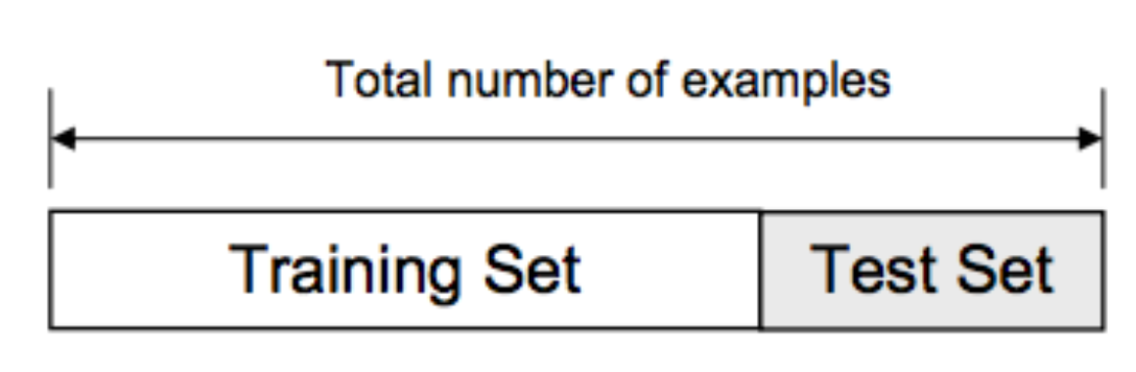
\includegraphics[width=.5\textwidth]{test_train.png}
	\caption{Training a model requires splitting data into a test set and a training set. \cite{kfold}}
	\label{test_train}
\end{figure}

This test set is untouched until the end when you evaluate the models performance on the data set. Thus, we already have a diminished data set when we are trying to train the model. There are useful methods to get the most out of your training set and tune hyperparameters. One such method is K-fold cross validation graphically depicted in Figure \ref{kfold}. KFold could be used to select $\lambda$ in Ridge regression, before training the model on the entire training set using the optimal $\lambda$.

\begin{figure}[ht]
	\centering
	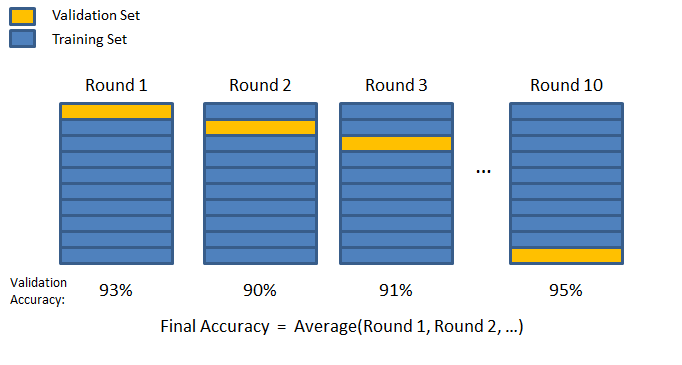
\includegraphics[width=.5\textwidth]{kfold.png}
	\caption{This figure depicts a K fold cross validation where $k=10$. \cite{kfold}}
	\label{kfold}
\end{figure}

$K$-fold cross validation takes the training data and partitions it into $K$ segments. It then trains the model on $K-1$ segments, and evaluates the fit of the model on the remaining segment. It runs $K$ rounds choosing a different validation segment each time. The average of the $K$ rounds is taken as the score. The entire process of splitting data and validating can be seen in Figure \ref{test_train_validate}.

\begin{figure}[ht]
	\centering
	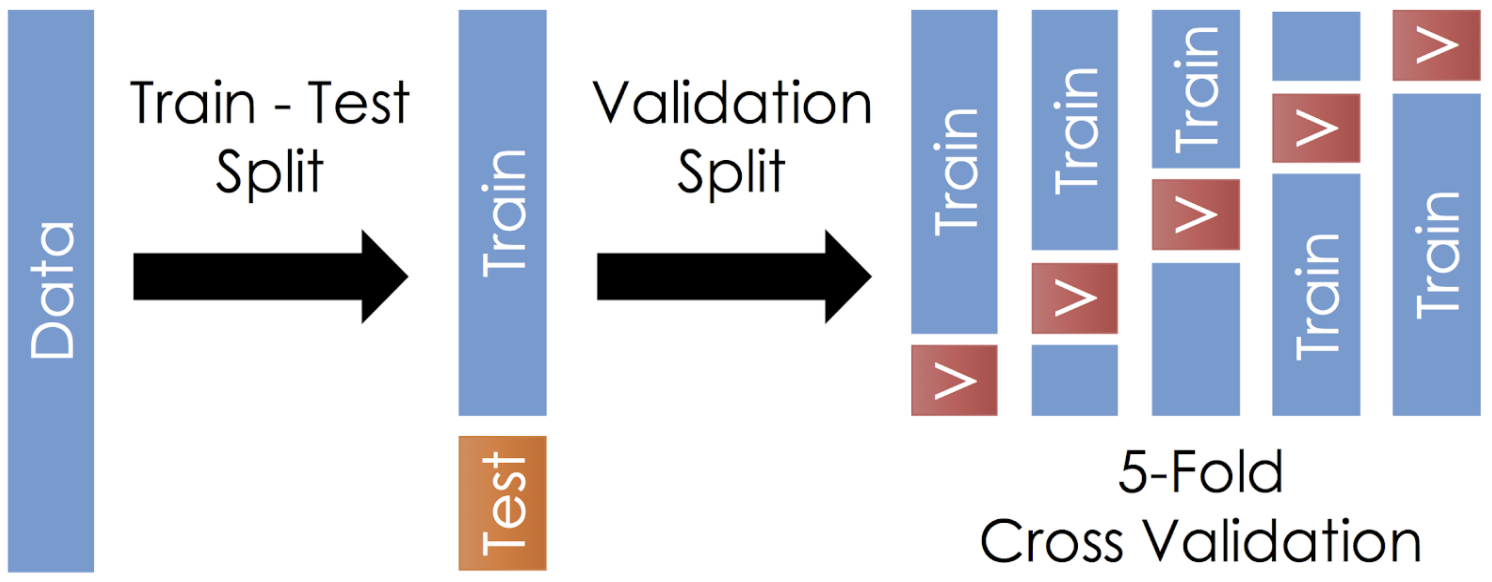
\includegraphics[width=.5\textwidth]{test_train_validate.png}
	\caption{This figure depicts the entire process of training a model. It demonstrates a $K$-fold cross validation where $k=10$. \cite{kfold2}}
	\label{test_train_validate}
\end{figure}

\clearpage 
\bibliographystyle{alpha}
\bibliography{litreview}
\end{document}
